\section{Detailed hyper-parameters on ImageNet-1K}

\myPara{PoolFormer}
On ImageNet-1K classification benchmark, we utilize the hyper-parameters shown in Table \ref{tab:hyperparameter} to train models in our paper. Based on the relation between batch size and learning rate in Table \ref{tab:hyperparameter}, we set the batch size as 4096 and learning rate as $4\times 10^{-3}$. For stochastic depth, following the original paper \cite{stochastic_depth}, we linearly increase the probability of dropping a layer from 0.0 for the bottom block to $d_r$ for the top block.

\begin{table*}[htbp]
\centering
\begin{tabular}{@{}l|ccccc@{}}
\toprule
 & \multicolumn{5}{c}{PoolFormer} \\ 
 & S12 & S24 & S36 & M36 & M48 \\
\midrule
Peak drop rate of stoch. depth $d_r$ & 0.1 & 0.1 & 0.2 & 0.3 & 0.4 \\
LayerScale initialization $\epsilon$ & $10^{-5}$ & $10^{-5}$ & $10^{-6}$ & $10^{-6}$ & $10^{-6}$ \\
\hline
Data augmentation & \multicolumn{5}{c}{AutoAugment} \\
Repeated Augmentation & \multicolumn{5}{c}{off} \\
Input resolution & \multicolumn{5}{c}{224} \\
Epochs & \multicolumn{5}{c}{300} \\
Warmup epochs & \multicolumn{5}{c}{5} \\
Hidden dropout & \multicolumn{5}{c}{0} \\
GeLU dropout & \multicolumn{5}{c}{0} \\
Classification dropout & \multicolumn{5}{c}{0} \\
Random erasing prob & \multicolumn{5}{c}{0.25} \\
EMA decay & \multicolumn{5}{c}{0} \\
Cutmix $\alpha$ & \multicolumn{5}{c}{1.0} \\
Mixup $\alpha$ & \multicolumn{5}{c}{0.8} \\
Cutmix-Mixup switch prob & \multicolumn{5}{c}{0.5} \\
Label smoothing & \multicolumn{5}{c}{0.1} \\
\tabincell{l}{Relation between peak learning \\ \qquad rate and batch size} & \multicolumn{5}{c}{$\mathrm{lr} = \frac{\mathrm{batch\_size}}{1024}\times 10^{-3}$} \\
Batch size used in the paper & \multicolumn{5}{c}{4096} \\
Peak learning rate used in the paper & \multicolumn{5}{c}{$4 \times 10^{-4}$} \\
Learning rate decay & \multicolumn{5}{c}{cosine} \\
Optimizer & \multicolumn{5}{c}{AdamW} \\
Adam $\epsilon$ & \multicolumn{5}{c}{1e-8} \\
Adam $(\beta_1, \beta_2)$ & \multicolumn{5}{c}{(0.9, 0.999)} \\
Weight decay & \multicolumn{5}{c}{0.05} \\
Gradient clipping & \multicolumn{5}{c}{None} \\
\bottomrule
\end{tabular}
\vspace{-2mm}
\caption{\textbf{Hyper-parameters for image classification on ImageNet-1K}
\label{tab:hyperparameter}
}
\end{table*}

\myPara{Hybrid Models}
We use the hyper-parameters for all models except for 
the hybrid models with token mixers of pooling and attention. 
For these hybrid models, we find that
they achieve much better performances
by setting batch size as 1024, 
learning rate as $10^{-3}$,
and normalization as
Layer Normalization \cite{layer_norm}.


\section{Training for longer epochs}
In our paper, PoolFormer models are trained for the default 300 epochs on ImageNet-1K. For DeiT \cite{deit}/ResMLP\cite{resmlp}, it is observed that the performance saturates after 400/800 epochs. Thus, we also conduct the experiments of training longer for PoolFormer-S12 and the results are shown in Table \ref{tab:long_epochs}. We observe that PoolFormer-S12 obtains saturated performance after around 2000 epochs with a top-1 accuracy improvement of 1.8\%. However, for fair comparison with other ViT/MLP-like models, we still train PoolFormers for 300 epochs by default.



%%%%%%%%% Table: longer epochs
\begin{table*}[t]
\centering
\setlength{\tabcolsep}{10pt}
\begin{tabular}{l c c c c c c c c}
\toprule
\# Epochs & 300 (default) & 400 & 500 & 1000 & 1500 & 2000 & 2500 & 3000 \\
\midrule
PoolFormer-S12 & 77.2 & 77.5 & 77.9 & 78.4 & 78.6 & 78.8 & 78.8 & 78.8 \\
\bottomrule
\end{tabular}
\vspace{-2mm}
\caption{\textbf{Performance of PoolFormer trained for different numbers of epochs}.}
\label{tab:long_epochs} 
\end{table*}

\section{Qualitative results}
We use Grad-CAM \cite{gradcam} to visualize the results of different models trained on ImageNet-1K. We find that although ResMLP \cite{resmlp} also activates some irrelevant parts, all models can locate the semantic objects. The activation parts of DeiT \cite{deit} and ResMLP \cite{resmlp} in the maps are more scattered, while those of RSB-ResNet \cite{resnet_improved, resnet} and PoolFormer are more gathered. 


\begin{figure*}[t]
    % \vspace{-3mm}
    \centering
    \begin{subfigure}[b]{0.19\textwidth}
        \centering
        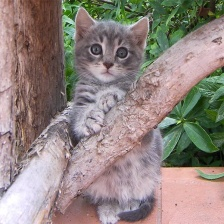
\includegraphics[width=1\textwidth]{figures/qualitative_results/ILSVRC2012_val_00023779_resize.JPEG}
        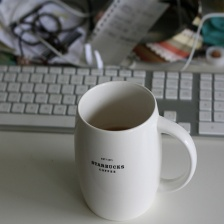
\includegraphics[width=1\textwidth]{figures/qualitative_results/ILSVRC2012_val_00016576_resize.JPEG}
        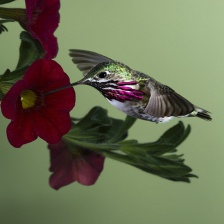
\includegraphics[width=1\textwidth]{figures/qualitative_results/ILSVRC2012_val_00005779_resize.JPEG}
        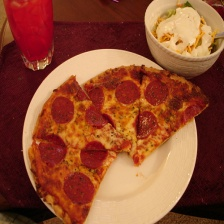
\includegraphics[width=1\textwidth]{figures/qualitative_results/ILSVRC2012_val_00018461_resize.JPEG}
    \end{subfigure}    
    \begin{subfigure}[b]{0.19\textwidth}
        \centering
        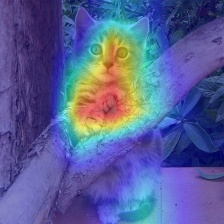
\includegraphics[width=1\textwidth]{figures/qualitative_results/ILSVRC2012_val_00023779_resnet50.JPEG}
        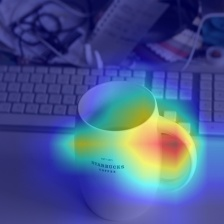
\includegraphics[width=1\textwidth]{figures/qualitative_results/ILSVRC2012_val_00016576_resnet50.JPEG}
        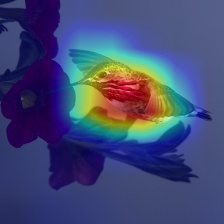
\includegraphics[width=1\textwidth]{figures/qualitative_results/ILSVRC2012_val_00005779_resnet50.JPEG}
        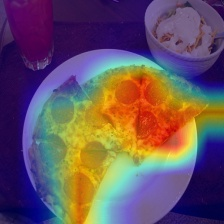
\includegraphics[width=1\textwidth]{figures/qualitative_results/ILSVRC2012_val_00018461_resnet50.JPEG}
    \end{subfigure}  
    \begin{subfigure}[b]{0.19\textwidth}
        \centering
        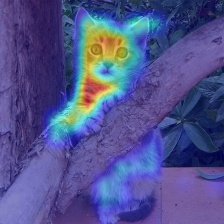
\includegraphics[width=1\textwidth]{figures/qualitative_results/ILSVRC2012_val_00023779_deit_small_patch16_224.JPEG}
        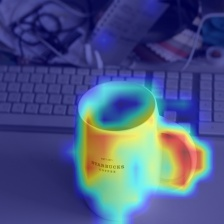
\includegraphics[width=1\textwidth]{figures/qualitative_results/ILSVRC2012_val_00016576_deit_small_patch16_224.JPEG}
        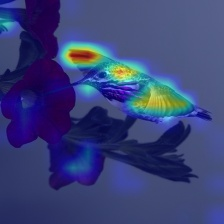
\includegraphics[width=1\textwidth]{figures/qualitative_results/ILSVRC2012_val_00005779_deit_small_patch16_224.JPEG}
        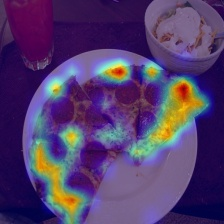
\includegraphics[width=1\textwidth]{figures/qualitative_results/ILSVRC2012_val_00018461_deit_small_patch16_224.JPEG}
    \end{subfigure}  
    \begin{subfigure}[b]{0.19\textwidth}
        \centering
        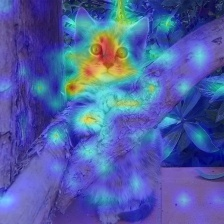
\includegraphics[width=1\textwidth]{figures/qualitative_results/ILSVRC2012_val_00023779_resmlp_24_224.JPEG}
        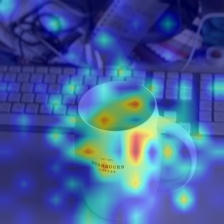
\includegraphics[width=1\textwidth]{figures/qualitative_results/ILSVRC2012_val_00016576_resmlp_24_224.JPEG}
        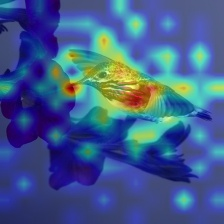
\includegraphics[width=1\textwidth]{figures/qualitative_results/ILSVRC2012_val_00005779_resmlp_24_224.JPEG}
        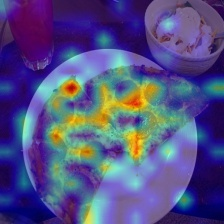
\includegraphics[width=1\textwidth]{figures/qualitative_results/ILSVRC2012_val_00018461_resmlp_24_224.JPEG}
    \end{subfigure}  
    \begin{subfigure}[b]{0.19\textwidth}
        \centering
        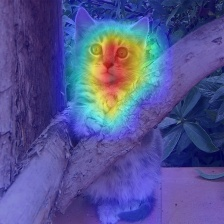
\includegraphics[width=1\textwidth]{figures/qualitative_results/ILSVRC2012_val_00023779_poolformer_s24.JPEG}
        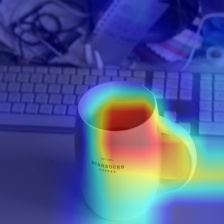
\includegraphics[width=1\textwidth]{figures/qualitative_results/ILSVRC2012_val_00016576_poolformer_s24.JPEG}
        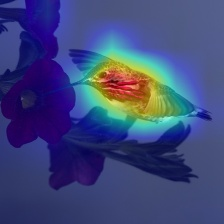
\includegraphics[width=1\textwidth]{figures/qualitative_results/ILSVRC2012_val_00005779_poolformer_s24.JPEG}
        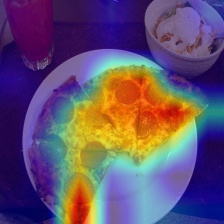
\includegraphics[width=1\textwidth]{figures/qualitative_results/ILSVRC2012_val_00018461_poolformer_s24.JPEG}
    \end{subfigure}  
    % \vspace{-7mm}
    \begin{center}
    	 ~~~~~~~Input\qquad \qquad \quad RSB-ResNet-50 \cite{resnet_improved} \qquad ~~ DeiT-small \cite{deit} \qquad ~~ ResMLP-S24 \cite{resmlp} \qquad ~~ PoolFormer-S24
    \end{center}  
    \caption{
        \label{grad_cam} Grad-CAM \cite{gradcam} activation maps of the models trained on ImageNet-1K. The visualized images are from validation set. 
    }
\end{figure*}
\section{Comparison between Layer Normalization and Modified Layer Normalization}
We modify Layer Normalization \cite{layer_norm} into Modified Layer Normalization (MNN). It computes the mean and variance along spatial and channel dimensions, compared with only channel dimension in vanilla Layer Normalization. The shape of learnable affine parameters of MLN keeps the same as that of Layer Normalization, \ie, $\mathbb{R^C}$. MLN can be implemented with GroupNorm API in PyTorch by setting the group number as 1. The comparison details are shown in Algorithm \ref{alg:norm}.



%%%%%%%%% Algorithm: modules
\begin{algorithm*}[t]
\caption{Comparison between Layer Normalization and Modified Layer Normalization, PyTorch-like Code}
\label{alg:norm}
\definecolor{codeblue}{rgb}{0.25,0.5,0.5}
\definecolor{codekw}{rgb}{0.85, 0.18, 0.50}
\lstset{
  backgroundcolor=\color{white},
  basicstyle=\fontsize{7.5pt}{7.5pt}\ttfamily\selectfont,
  columns=fullflexible,
  breaklines=true,
  captionpos=b,
  commentstyle=\fontsize{7.5pt}{7.5pt}\color{codeblue},
  keywordstyle=\fontsize{7.5pt}{7.5pt}\color{codekw},
}
\begin{lstlisting}[language=python]
import torch.nn as nn


class LayerNormChannel(nn.Module):
    """
    Vanilla Layer Normalization normalizes vectors along channel dimension.
    Input: tensor in shape [B, C, H, W].
    """
    def __init__(self, num_channels, eps=1e-05):
        super().__init__()
        # The shape of  learnable affine parameters is [num_channels, ].
        self.weight = nn.Parameter(torch.ones(num_channels))
        self.bias = nn.Parameter(torch.zeros(num_channels))
        self.eps = eps

    def forward(self, x):
        u = x.mean(1, keepdim=True) # Compute the means along channel dimension.
        s = (x - u).pow(2).mean(1, keepdim=True) # Compute the variances along channel dimension.
        x = (x - u) / torch.sqrt(s + self.eps)
        x = self.weight.unsqueeze(-1).unsqueeze(-1) * x \
            + self.bias.unsqueeze(-1).unsqueeze(-1)
        return x
        

class ModifiedLayerNorm(nn.Module):
    """
    Modified Layer Normalization normalizes vectors along channel dimension and spatial dimensions.
    Input: tensor in shape [B, C, H, W]
    """
    def __init__(self, num_channels, eps=1e-05):
        super().__init__()
        # The shape of  learnable affine parameters is also [num_channels, ], keeping the same as vanilla Layer Normalization.
        self.weight = nn.Parameter(torch.ones(num_channels))
        self.bias = nn.Parameter(torch.zeros(num_channels))
        self.eps = eps

    def forward(self, x):
        u = x.mean([1, 2, 3], keepdim=True) # Compute the mean along channel dimension and spatial dimensions.
        s = (x - u).pow(2).mean([1, 2, 3], keepdim=True) # Compute the variance along channel dimension and spatial dimensions.
        x = (x - u) / torch.sqrt(s + self.eps)
        x = self.weight.unsqueeze(-1).unsqueeze(-1) * x \
            + self.bias.unsqueeze(-1).unsqueeze(-1)
        return x
        

# Modified Layer Normalization can also be implemented using GroupNorm API in PyTorch by setting the group number as 1.        
class ModifiedLayerNorm(nn.GroupNorm):
    """
    Modified Layer Normalization implemented by Group Normalization with 1 group.
    Input: tensor in shape [B, C, H, W]
    """
    def __init__(self, num_channels, **kwargs):
        super().__init__(1, num_channels, **kwargs)
\end{lstlisting}
\end{algorithm*}


\section{Code in PyTorch}
We provide the PyTorch-like code in Algorithm \ref{alg:module} associated with the modules used in the PoolFormer block. Algorithm~\ref{alg:block} further shows the PoolFormer block built with these modules. 


%%%%%%%%% Algorithm: modules
\begin{algorithm*}[t]
\caption{Modules for PoolFormer block, PyTorch-like Code}
\label{alg:module}
\definecolor{codeblue}{rgb}{0.25,0.5,0.5}
\definecolor{codekw}{rgb}{0.85, 0.18, 0.50}
\lstset{
  backgroundcolor=\color{white},
  basicstyle=\fontsize{7.5pt}{7.5pt}\ttfamily\selectfont,
  columns=fullflexible,
  breaklines=true,
  captionpos=b,
  commentstyle=\fontsize{7.5pt}{7.5pt}\color{codeblue},
  keywordstyle=\fontsize{7.5pt}{7.5pt}\color{codekw},
}
\begin{lstlisting}[language=python]
import torch.nn as nn


class ModifiedLayerNorm(nn.GroupNorm):
    """
    Modified Layer Normalization implemented by Group Normalization with 1 group.
    Input: tensor in shape [B, C, H, W]
    """
    def __init__(self, num_channels, **kwargs):
        super().__init__(1, num_channels, **kwargs)


class Pooling(nn.Module):
    """
    Implementation of pooling for PoolFormer
    --pool_size: pooling size
    Input: tensor with shape [B, C, H, W]
    """
    def __init__(self, pool_size=3):
        super().__init__()
        self.pool = nn.AvgPool2d(
            pool_size, stride=1, padding=pool_size//2, count_include_pad=False)

    def forward(self, x):
        # Subtraction of the input itself is added 
        # since the block already has a residual connection.
        return self.pool(x) - x


class Mlp(nn.Module):
    """
    Implementation of MLP with 1*1 convolutions.
    Input: tensor with shape [B, C, H, W]
    """
    def __init__(self, in_features, hidden_features=None, 
                 out_features=None, act_layer=nn.GELU, drop=0.):
        super().__init__()
        out_features = out_features or in_features
        hidden_features = hidden_features or in_features
        self.fc1 = nn.Conv2d(in_features, hidden_features, 1)
        self.act = act_layer()
        self.fc2 = nn.Conv2d(hidden_features, out_features, 1)
        self.drop = nn.Dropout(drop)
        self.apply(self._init_weights)

    def _init_weights(self, m):
        if isinstance(m, nn.Conv2d):
            trunc_normal_(m.weight, std=.02)
            if m.bias is not None:
                nn.init.constant_(m.bias, 0)

    def forward(self, x):
        x = self.fc1(x)
        x = self.act(x)
        x = self.drop(x)
        x = self.fc2(x)
        x = self.drop(x)
        return x
\end{lstlisting}
\end{algorithm*}


%%%%%%%%% Algorithm: block
\begin{algorithm*}[t]
\caption{PoolFormer block, PyTorch-like Code}
\label{alg:block}
\definecolor{codeblue}{rgb}{0.25,0.5,0.5}
\definecolor{codekw}{rgb}{0.85, 0.18, 0.50}
\lstset{
  backgroundcolor=\color{white},
  basicstyle=\fontsize{7.5pt}{7.5pt}\ttfamily\selectfont,
  columns=fullflexible,
  breaklines=true,
  captionpos=b,
  commentstyle=\fontsize{7.5pt}{7.5pt}\color{codeblue},
  keywordstyle=\fontsize{7.5pt}{7.5pt}\color{codekw},
}
\begin{lstlisting}[language=python]
import torch.nn as nn


class PoolFormerBlock(nn.Module):
    """
    Implementation of one PoolFormer block.
    --dim: embedding dim
    --pool_size: pooling size
    --mlp_ratio: mlp expansion ratio
    --act_layer: activation
    --norm_layer: normalization
    --drop: dropout rate
    --drop path: Stochastic Depth, 
        refer to https://arxiv.org/abs/1603.09382
    --use_layer_scale, --layer_scale_init_value: LayerScale, 
        refer to https://arxiv.org/abs/2103.17239
    """
    def __init__(self, dim, pool_size=3, mlp_ratio=4., 
                 act_layer=nn.GELU, norm_layer=ModifiedLayerNorm, 
                 drop=0., drop_path=0., 
                 use_layer_scale=True, layer_scale_init_value=1e-5):

        super().__init__()

        self.norm1 = norm_layer(dim)
        self.token_mixer = Pooling(pool_size=pool_size)
        self.norm2 = norm_layer(dim)
        mlp_hidden_dim = int(dim * mlp_ratio)
        self.mlp = Mlp(in_features=dim, hidden_features=mlp_hidden_dim, 
                       act_layer=act_layer, drop=drop)

        # The following two techniques are useful to train deep PoolFormers.
        self.drop_path = DropPath(drop_path) if drop_path > 0. \
            else nn.Identity()
        self.use_layer_scale = use_layer_scale
        if use_layer_scale:
            self.layer_scale_1 = nn.Parameter(
                layer_scale_init_value * torch.ones(dim), requires_grad=True)
            self.layer_scale_2 = nn.Parameter(
                layer_scale_init_value * torch.ones(dim), requires_grad=True)

    def forward(self, x):
        if self.use_layer_scale:
            x = x + self.drop_path(
                self.layer_scale_1.unsqueeze(-1).unsqueeze(-1)
                * self.token_mixer(self.norm1(x)))
            x = x + self.drop_path(
                self.layer_scale_2.unsqueeze(-1).unsqueeze(-1)
                * self.mlp(self.norm2(x)))
        else:
            x = x + self.drop_path(self.token_mixer(self.norm1(x)))
            x = x + self.drop_path(self.mlp(self.norm2(x)))
        return x
\end{lstlisting}
\end{algorithm*}
